\chapter{Phase Transitions}

Phase transitions are among the most striking manifestations of collective behavior in statistical physics.
They represent abrupt qualitative changes in the macroscopic state of matter that arise from the smooth variation of a few external control parameters, such as temperature, pressure, or magnetic field.
At the microscopic level, these transitions emerge from the cooperative dynamics of a very large number of interacting degrees of freedom, leading to singularities in thermodynamic quantities and to the spontaneous breaking of symmetries.

In this chapter, we develop the thermodynamic and statistical foundations needed to describe and classify phase transitions.
We begin by introducing the concept of a \textit{phase diagram}, which organizes the possible equilibrium states of a system and identifies coexistence regions where two or more phases can be in equilibrium.
We then derive the \textit{Clausius--Clapeyron equation}, which provides a quantitative description of coexistence curves and the relation between intensive thermodynamic variables along phase boundaries.

Next, we discuss the \textit{classification of phase transitions} according to the nature of the non--analyticity of the free energy, distinguishing between first--order transitions, characterized by discontinuities in first derivatives (such as latent heat or density jumps), and continuous or higher--order transitions, where thermodynamic quantities remain continuous but their derivatives diverge.
This classification naturally leads to the study of critical phenomena and universality.

Finally, to illustrate how these ideas emerge from microscopic models, we consider the paradigmatic example of the \textit{Ising model}.
Despite its simplicity, this lattice model captures the essential features of cooperative ordering and provides a concrete realization of a continuous phase transition, allowing us to connect the abstract thermodynamic description with a statistical–mechanical one.

Throughout this chapter, our aim is to bridge the phenomenological thermodynamics of phase transitions with their microscopic statistical interpretation, highlighting how non--analytic behavior in macroscopic observables originates from the collective organization of microscopic states.

\section{Phase Diagrams}

A classical fluid can exist in different phases—solid, liquid, and gas—depending on its temperature \(T\) and pressure \(p\). In the \(p-T\) diagram, these phases occupy distinct regions separated by phase boundaries, along which two phases can coexist in equilibrium.

\paragraph{Coexistence lines and triple point.}
In a phase diagram, the \textit{coexistence lines} (or phase boundaries) represent the set of thermodynamic states where two phases of the same substance can coexist in equilibrium. Along each line, the temperature, pressure, and chemical potential of the two phases are equal,
\[
    T_1 = T_2, \qquad p_1 = p_2, \qquad \mu_1 = \mu_2,
\]
ensuring that the transformation can occur reversibly under constant thermodynamic conditions.
These three coexistence lines meet at a unique point in the \(p\)--\(T\) plane called the \textit{triple point}, where solid, liquid, and vapor coexist simultaneously in thermodynamic equilibrium.
At this point, the equality of temperature, pressure, and chemical potential extends to all three phases,
\[
    T_\mathrm{s} = T_\mathrm{l} = T_\mathrm{v}, \qquad
    p_\mathrm{s} = p_\mathrm{l} = p_\mathrm{v}, \qquad
    \mu_\mathrm{s} = \mu_\mathrm{l} = \mu_\mathrm{v},
\]
so that mass can be exchanged among them without altering the macroscopic state of the system.
The triple point thus defines a fundamental reference in thermodynamics, often used for the calibration of temperature and pressure scales.

\begin{figure}[H]
    \begin{minipage}[b]{0.55\textwidth}
        \includegraphics[width=0.9\textwidth]{img/phase_diag_classical_fluid.png}
        \caption{A schematic phase diagram showing different phases of a classical fluid, with regions of solid, liquid, and gas separated by phase boundaries. Critical points and triple points are also indicated, along with the coexistence curves.}
    \end{minipage}
    \hfill
    \begin{minipage}[b]{0.4\textwidth}
        The solid–liquid line marks the conditions of melting and freezing, while the liquid–vapor line corresponds to vaporization and condensation. The solid–vapor line instead represents sublimation and deposition processes. All three boundaries meet at the triple point, where the three phases coexist simultaneously in thermodynamic equilibrium. The liquid–vapor coexistence curve terminates at the critical point, beyond which the distinction between liquid and gas disappears and the substance forms a supercritical fluid. Each phase transition involves a discontinuous change in certain thermodynamic properties, such as density or enthalpy, and can be associated with a latent heat exchange between the phases.
    \end{minipage}
\end{figure}

\paragraph{Critical point and superfluidity.}
The \textit{critical point} marks the upper end of the liquid--vapor coexistence curve in the \(p\)--\(T\) diagram. At this point, the distinction between liquid and gas disappears: the densities of the two phases become equal, and the surface tension vanishes.
Beyond the critical point, the substance forms a \textit{supercritical fluid}, a single homogeneous phase that exhibits properties intermediate between those of a liquid and a gas, such as high diffusivity combined with a relatively large density. The system does not dissipate energy from friction as a normal fluid would, allowing it to flow without viscosity.
The critical point is characterized by continuous (second--order) phase transition behavior, where response functions such as compressibility and heat capacity diverge according to universal critical exponents.

In certain quantum fluids, such as liquid helium--4, a different kind of continuous phase transition occurs at very low temperatures, leading to the onset of \textbf{superfluidity}.
\begin{figure}[H]
    \begin{minipage}[b]{0.4\textwidth}
        Below the so--called $\lambda$--point (at \(T_\lambda \approx 2.17~\mathrm{K}\) under saturated vapor pressure), helium--4 undergoes a transition from the normal liquid phase (He~I) to the superfluid phase (He~II).
        The superfluid phase exhibits remarkable macroscopic quantum phenomena, including the absence of viscosity, the ability to flow through extremely narrow capillaries, and the quantization of vorticity.
        Although both the critical point and the superfluid transition correspond to continuous changes in the state of the system, they originate from different microscopic mechanisms: the former arises from the disappearance of density fluctuations at large scales, while the latter emerges from Bose--Einstein condensation of helium atoms.
    \end{minipage}
    \hfill
    \begin{minipage}[b]{0.55\textwidth}
        \includegraphics[width=0.9\textwidth]{img/phase_diag_4He.png}
        \caption{Schematic phase diagram of liquid helium-4, showing solid, liquid, gas, and superfluid regions separated by phase boundaries. Coexistence curves are indicated where appropriate, while the boundary between the liquid and superfluid phases is shown for reference, even though this transition is continuous.}
    \end{minipage}
\end{figure}

\subsection{Clausius--Clapeyron Equation}

Consider a system at equilibrium along a phase coexistence line between two phases, denoted \(\alpha\) and \(\beta\).
The Gibbs free energy of the system is
\[
    G(T,p) = \mu N,
\]
where \(\mu\) is the chemical potential and \(N\) the number of particles.
Per particle, the Gibbs free energy is
\[
    g = \frac{G}{N} = \mu.
\]
At equilibrium along the coexistence line, the chemical potentials of the two phases are equal:
\[
    \mu_\alpha(T,p) = \mu_\beta(T,p) \quad \implies \quad g_\alpha(T,p) = g_\beta(T,p).
\]

Differentiating both sides along the coexistence line gives
\[
    d\mu_\alpha = d\mu_\beta.
\]

Using the thermodynamic identity for the Gibbs free energy per particle,
\[
    d\mu = -s \, dT + v \, dp,
\]
where \(s\) and \(v\) are the molar entropy and molar volume, respectively, we obtain
\[
    - s_\alpha \, dT + v_\alpha \, dp = - s_\beta \, dT + v_\beta \, dp.
\]
Now we can differentiate with respect to temperature:
\[
    \frac{\d{\mu}}{\d{T}} = \left(\frac{\partial \mu}{\partial T}\right)_p + \left(\frac{\partial \mu}{\partial p}\right)_T \frac{\d{p}}{\d{T}} = -s + v \frac{dp}{dT},
\]
and rewriting this, the slope of the coexistence curve in the \(p\)--\(T\) plane is
\[
    \frac{dp}{dT} = \frac{s_\beta - s_\alpha}{v_\beta - v_\alpha} = \frac{\Delta s}{\Delta v}.
\]
Introducing the \textbf{latent heat} \(q\) per mole, which is the heat absorbed or released during the phase transition at constant temperature and pressure, we have
\[
    q = T \, \Delta s.
\]
Substituting this relation into the previous expression, we obtain the \textbf{Clausius--Clapeyron equation}:
\[
    \frac{dp}{dT} = \frac{q}{T \, \Delta v}.
\]

This equation provides a fundamental link between measurable thermodynamic quantities along the coexistence line: the slope of the phase boundary is determined by the latent heat of the transition and the change in molar volume between the two phases.

\section{Classification of Phase Transitions}

Phase transitions can be broadly divided into two main categories: \textit{first--order} and \textit{continuous} (or \textit{second--order}) transitions, depending on the nature of the discontinuities that appear in the thermodynamic description of the system.

Historically, phase transitions were classified according to the \textit{Ehrenfest scheme}, which identified the order of the transition with the lowest derivative of the Gibbs free energy that exhibits a discontinuity.
Although this classification remains conceptually useful, it has been largely superseded by a more general framework developed in modern statistical mechanics, which textitasizes critical behavior and universality near continuous transitions.

\subsection{First--Order Phase Transitions}
First--order phase transitions are characterized by a discontinuous change in the first derivatives of the free energy with respect to the thermodynamic variables.
In particular, quantities such as volume or entropy experience finite jumps at the transition point.
These discontinuities imply the exchange of a finite amount of heat at constant temperature and pressure, known as the \textit{latent heat} of the transition:
\[
    L = T \, \Delta s,
\]
where \(\Delta s\) is the entropy difference between the two coexisting phases.
First--order transitions are accompanied by the coexistence of phases and occur along well-defined lines in the \(p\)--\(T\) plane.
Typical examples include the melting of a solid, the vaporization of a liquid, and the sublimation of a solid into vapor.

\subsection{Continuous Phase Transitions}
Continuous (or second--order) phase transitions are characterized by the continuity of the first derivatives of the free energy, while higher-order derivatives become discontinuous or diverge.
No latent heat is involved, and the transition occurs smoothly, often associated with the emergence of long-range correlations and critical fluctuations.
Near the critical point, the system exhibits \textit{scale invariance} and \textit{universal behavior}, where macroscopic properties depend only on general features such as symmetry and dimensionality, rather than on microscopic details.
Examples include the liquid--gas critical point and the superfluid transition in helium--4.

\begin{remark}
    The presence or absence of latent heat provides a clear thermodynamic signature distinguishing first--order from continuous phase transitions.
    In first--order transitions, the system absorbs or releases a finite amount of energy to reorganize its microscopic structure, while in continuous transitions, this reorganization occurs gradually, with thermodynamic quantities varying smoothly but response functions (such as heat capacity or compressibility) diverging near the critical point.
\end{remark}

\section{Discontinuities and Phase Transitions}

Phase transitions are intimately connected with the analytic structure of the partition function.
For finite systems, \( \mathcal{Z}_N(\lambda) \) is an analytic function of its parameters, so true singularities cannot occur.
However, the distribution of its zeros in the complex plane reveals where non--analytic behavior may emerge in the thermodynamic limit.

This analytic mechanism was first formalized by Lee and Yang in a pair of theorems that establish both the existence and the analyticity properties of the thermodynamic potential in the complex plane of the control parameter.

\begin{theorem}[Lee--Yang I | Existence of the thermodynamic limit]
    Consider a system of \(N\) interacting particles with potential energy \(U_N\) satisfying the stability bound
    \[
        U_N \geq - B N , \qquad B > 0,
    \]
    and contained in a volume \(V\) whose boundary increases no faster than \(V^{2/3}\).
    Then, for any complex fugacity \(z = e^{\beta \mu}\), the limit
    \[
        \Psi(z,v,T) = \lim_{V \to \infty} \frac{1}{V} \log \mathcal{Z}(z,V,T)
    \]
    exists and defines a continuous, monotonically increasing function of \(z \in \mathbb{R}^+\).
\end{theorem}

\begin{theorem}[Lee--Yang II | Analyticity and distribution of zeros]
    Let \(R\) be an open subset of the complex \(z\)--plane containing a portion of the positive real axis.
    If, for all finite \(V\) and \(T\), the grand partition function \( \mathcal{Z}(z,V,T) \) has no zeros in \(R\),
    then the sequence \( (\log \mathcal{Z}(z,V,T))/V \) converges uniformly as \( V \to \infty \) in any closed subset of \(R\),
    and therefore the thermodynamic potential \( \Psi(z,v,T) \) is analytic in \(R\).
\end{theorem}

The two results together imply that a phase transition can only occur if, in the thermodynamic limit, a locus of zeros of the finite--volume partition function \(\mathcal{Z}(z,V,T)\) approaches the positive real axis.
The point \(z_c\) where this accumulation occurs divides the real axis into distinct analytic regions, corresponding to different thermodynamic phases.
At \(z = z_c\), the potential \( \Psi(z,v,T) \) remains continuous but becomes non--analytic:
a cusp singularity corresponds to a first--order phase transition, while higher--order singularities describe continuous phase transitions.

\begin{remark}
    The celebrated \textit{Lee--Yang circle theorem} is a special case of this general framework, proved for the ferromagnetic Ising model, where all zeros of the partition function in the complex fugacity plane \( z = e^{-2\beta h} \) lie on the unit circle \( |z| = 1 \).
    In more general systems, such as lattice gases or fluids with realistic interactions, the zeros no longer lie on a perfect circle, yet their accumulation and contact with the real axis remain the universal analytic mechanism underlying phase transitions.
\end{remark}

To illustrate the qualitative content of the \textbf{first Lee--Yang theorem}, let us consider a system described by a mean--field Hamiltonian, for which the grand partition function can be written as a polynomial of finite degree \( N \) in the complex fugacity \( z \). Starting from the canonical partition function of a system with Hamiltonian
\[
    \mathcal{H} = \sum_i \frac{p_i^2}{2m} + U_N(q_1, \dots, q_N),
\]
we can integrate over the momenta and separate the purely configurational contribution:
\[
    Z_N = \int_V \! \mathrm{d}\Omega \, e^{-\beta \mathcal{H}}
    = \frac{Q_N}{N!\,\lambda_{\mathrm{th}}^{3N}},
    \qquad
    Q_N = \int \prod_i \mathrm{d}^3q_i \, e^{-\beta U_N(q_1,\dots,q_N)}.
\]
Here, \( Q_N \) encodes the interaction between particles, while the prefactor
\( 1/(N!\lambda_{\mathrm{th}}^{3N}) \) represents the contribution of indistinguishability and kinetic energy.

Hence, the grand partition function of the system reads
\[
    \mathcal{Z}_N(z)
    = \sum_{n=0}^N \frac{z^n Q_n}{n!\,\lambda_{\mathrm{th}}^{3n}}
    = \sum_{n=0}^N a_n z^n,
    \qquad a_n > 0 \ \forall n.
\]
At finite \( N \), this is a polynomial in \( z \) with positive coefficients.
Even before taking the thermodynamic limit, this already implies that the zeros of
\( \mathcal{Z}_N(z) \) cannot lie on the positive real axis, since all the coefficients
of the polynomial are strictly positive. Therefore, for any finite system, the grand
partition function is analytic and positive for \( z \in \mathbb{R}^+ \).

To examine whether the thermodynamic limit exists, we must ensure that the series
remains convergent as \( N \to \infty \). We assume, as in the standard proof, that
the interaction potential is bounded from below by a function linear in \( N \):
\[
    U_N \ge -K N, \qquad K > 0.
\]
This lower bound guarantees the system’s stability: the energy cannot decrease
faster than linearly with the number of particles. From this condition, it follows that
\[
    e^{-\beta U_N} \le e^{\beta K N}.
\]
Using this inequality, we can bound the configurational integral:
\[
    Q_N \le V^N e^{\beta K N}.
\]
Substituting this estimate into the series for \( \mathcal{Z}_N(z) \), we find
\[
    \mathcal{Z}_N(z)
    \le \sum_{n=0}^N
    \frac{1}{n!}
    \left( \frac{z V e^{\beta K}}{\lambda_{\mathrm{th}}^{3}} \right)^n
    \xrightarrow{N\to\infty}
    \exp\!\left( \frac{z V e^{\beta K}}{\lambda_{\mathrm{th}}^{3}} \right).
\]
The thermodynamic limit is therefore well defined: the grand partition function
approaches a continuous, positive, monotonically increasing function for all
\( z \in \mathbb{R}^+ \).

In summary, the essential point of the first Lee--Yang theorem is that,
under the assumption of thermodynamic stability (i.e., a potential bounded
from below), the grand partition function \( \mathcal{Z}(z) \) is analytic
for positive real fugacity and its thermodynamic limit is well defined.

The \textbf{second Lee--Young theorem} help us understand how singularities can appear in the thermodynamic limit: we have to focus on the logarithm of the grand partition function. All thermodynamic quantities, such as pressure, density, or free energy, are obtained from derivatives of
\[
    \Phi = \log \mathcal{Z}.
\]
Therefore, the zeros of \( \mathcal{Z} \) correspond to singularities of \( \Phi \), and thus to possible singularities of thermodynamic observables. In other words, any non-analytic behaviour of macroscopic quantities must originate from points in the complex fugacity plane where \( \mathcal{Z} = 0 \).

From the previous discussion, we know that at finite \( N \) the grand partition function
\[
    \mathcal{Z}_N(z) = \sum_{n=0}^N a_n z^n, \qquad a_n > 0,
\]
is a polynomial with strictly positive coefficients.
\begin{figure}[H]
    \begin{minipage}[b]{0.55\textwidth}
        \begin{center}
            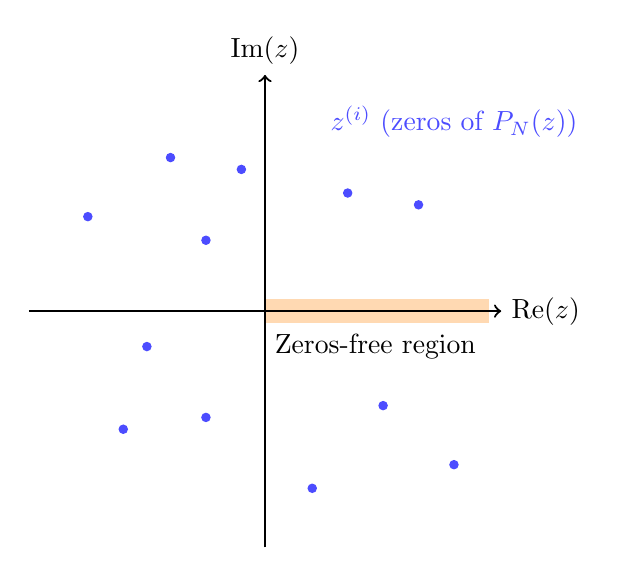
\begin{tikzpicture}[scale=1.5]
                \fill[orange!30] (0,-0.1) rectangle (1.9,0.1);
                \node[right] at (0,-0.3) {Zeros-free region};

                \draw[->, thick] (-2,0) -- (2,0) node[right] {Re$(z)$};
                \draw[->, thick] (0,-2) -- (0,2) node[above] {Im$(z)$};

                \foreach \x/\y in {-1.5/0.8, -0.5/0.6, -1/-0.3, -1.2/-1.0, -0.8/1.3, -0.5/-0.9, -0.2/1.2,
                        0.4/-1.5, 0.7/1.0, 1.0/-0.8, 1.3/0.9, 1.6/-1.3} {
                        \filldraw[blue!70] (\x,\y) circle (1pt);
                    }

                \node[blue!70] at (1.6,1.6) {$z^{(i)}$ (zeros of $P_{N}(z)$)};
            \end{tikzpicture}
        \end{center}
    \end{minipage}
    \hfill
    \begin{minipage}[b]{0.4\textwidth}
        By the fundamental theorem of algebra, it possesses \( N \) complex zeros, but since all coefficients are positive, none of these zeros can lie on the positive real axis. As a result, for any finite \( N \), \( \mathcal{Z}_N(z) \) is analytic and strictly positive for real positive \( z \), which means that no true phase transition can occur in a system of finite size. The partition function, and hence all thermodynamic functions derived from it, remain smooth and differentiable.
    \end{minipage}
\end{figure}


\begin{figure}[H]
    \begin{minipage}[b]{0.4\textwidth}
        However, the situation changes qualitatively in the thermodynamic limit \( N, V \to \infty \) with fixed density. As \( N \) increases, the zeros of \( \mathcal{Z}_N(z) \) in the complex \( z \)-plane can become denser and may start to accumulate along certain curves. In this limit, the set of zeros can form continuous lines or regions in the complex plane.
    \end{minipage}
    \hfill
    \begin{minipage}[b]{0.55\textwidth}
        \begin{center}

            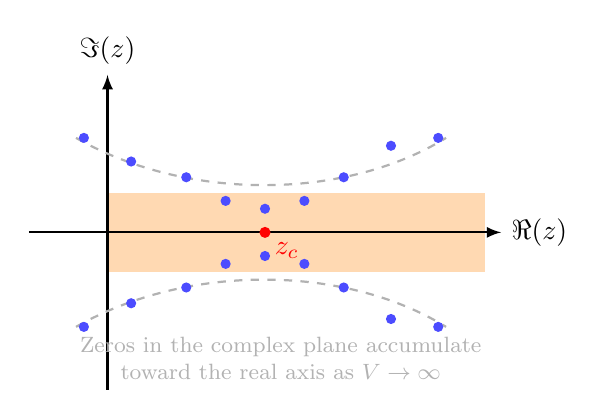
\begin{tikzpicture}[font=\sffamily, >=latex]
                \fill[orange!30] (-2,-0.5) rectangle (2.8,0.5);

                \tikzset{
                    axis/.style = {->, thick},
                    zero/.style = {circle, fill=blue!70, inner sep=1.3pt},
                    ghostzero/.style = {circle, fill=black!40, inner sep=1pt},
                    acc/.style = {dashed, thick},
                }

                \draw[axis] (-3,0) -- (3,0) node[right] {$\Re (z)$};
                \draw[axis] (-2,-2) -- (-2,2) node[above] {$\Im (z)$};

                \draw[acc, gray!60] (-2.4,1.2) .. controls (-1.0,0.4) and (1.0,0.4) .. (2.3,1.2);
                \draw[acc, gray!60] (-2.4,-1.2) .. controls (-1.0,-0.4) and (1.0,-0.4) .. (2.3,-1.2);

                \foreach \x/\y in {-2.3/1.2, -1.7/0.9, -1.0/0.7, -0.5/0.4, 0.0/0.3, 0.5/0.4, 1.0/0.7, 1.6/1.1, 2.2/1.2}{
                        \node[zero] at (\x,\y) {};
                        \node[zero] at (\x,-\y) {};
                    }

                \fill[red] (0,0) circle (2pt);
                \node[below right, red] at (0,0) {$z_c$};

                \node[align=center, font=\footnotesize, gray!60] at (0.2,-1.6)
                {Zeros in the complex plane accumulate\\
                    toward the real axis as $V \to \infty$};

            \end{tikzpicture}
        \end{center}
    \end{minipage}
\end{figure}

If such a line of zeros \(z^{(i)}\) approaches the positive real axis, then the logarithm of the partition function, \( \Phi(z) = \log \mathcal{Z}(z)\), becomes non-analytic at the point \(z_c\) where the accumulation occurs:
\[
    z^{(i)} \in \mathbb{C} - \mathbb{R}^+, \quad z^{(i)} \xrightarrow{N\to \infty} z_c \in \mathbb{R}^+.
\]
This non-analyticity is precisely what we interpret as a phase transition.

Hence, the second Lee--Yang theorem provides a qualitative explanation for the origin of thermodynamic singularities: the partition function itself is always analytic for finite systems, but as the system size grows, its zeros in the complex fugacity plane can condense and ``pinch'' the real axis. The point where this happens marks the emergence of a macroscopic phase transition.

\begin{remark}
    In practice, even though the Lee--Yang theorems show that true non--analyticities can only appear strictly in the thermodynamic limit, real systems with a large but finite number of particles can still exhibit apparent phase transitions.
    For instance, a small bottle of water can freeze or boil sharply, even though it contains a finite (and thus analytic) number of degrees of freedom. This happens because, for macroscopic \(N\), the zeros of the partition function \(\mathcal{Z}_N(z)\) already lie extremely close to the real axis.
    As a consequence, the derivatives of \(\log \mathcal{Z}_N\) can vary very rapidly near those quasi--singular points, producing an abrupt but smooth crossover that is experimentally indistinguishable from a genuine discontinuity.
\end{remark}

\section{Heisemberg and Ising Model}

The Ising model represents one of the simplest yet most profound models in statistical mechanics.
It captures the essential mechanism behind magnetic ordering, spontaneous symmetry breaking, and the appearance of phase transitions in systems composed of many interacting constituents.
Although originally conceived to describe ferromagnetism, its conceptual framework extends to a wide class of collective phenomena, from lattice gases to binary mixtures and neural networks.

In this chapter, we will start by analyzing the simplest possible case: a system of magnetic moments embedded in a crystalline solid lattice, each associated with a magnetic moment, but \textit{without} any interaction between the spins. This will be done with the Heisemberg model, which accounts for \(3D\)-spins.
This non-interacting model describes a collection of distinguishable atoms with magnetic moments oscillating in a thermal bath, where the total energy is determined solely by their coupling with an external magnetic field.
Such a system corresponds to a \textit{paramagnet}, and its behavior can be completely understood within the framework of classical equilibrium statistical mechanics.

We will then introduce interactions between neighboring magnetic moments, which tend to align or anti-align depending on the sign of the coupling constant.
It is precisely this introduction of spin--spin interaction that gives rise to the emergence of cooperative behavior and, eventually, to a \textit{phase transition} between the paramagnetic and ferromagnetic phases.
Thus, the Ising model clearly illustrates how the collective properties of matter — such as magnetization and critical phenomena — arise from the interplay between microscopic interactions and thermal fluctuations.

\subsection{Non-interacting Magnetic Spins}

We consider a crystalline solid consisting of \(N\) atoms arranged on a regular lattice of fixed volume \(V\) and temperature \(T\).
Each lattice site hosts a single atom, whose center of mass is bound to oscillate around its equilibrium position due to thermal vibrations.

\begin{figure}[H]
    \begin{minipage}[b]{0.35\textwidth}
        \centering
        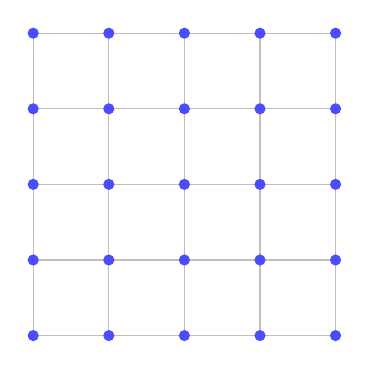
\begin{tikzpicture}[scale=1.2]
            \def\L{0.8}
            \def\nx{4}
            \def\ny{4}

            \foreach \i in {0,...,\nx}{
                    \foreach \j in {0,...,\ny}{
                            \ifnum\i<\nx
                                \draw[gray!50] (\i*\L, \j*\L) -- ({(\i+1)*\L}, \j*\L);
                            \fi
                            \ifnum\j<\ny
                                \draw[gray!50] (\i*\L, \j*\L) -- (\i*\L, {(\j+1)*\L});
                            \fi
                            \filldraw[blue!70] (\i*\L, \j*\L) circle (1.5pt);
                        }
                }
        \end{tikzpicture}
    \end{minipage}
    \hfill
    \begin{minipage}[b]{0.6\textwidth}
        For the purpose of studying magnetic properties, we assume that these translational vibrations are small and can be effectively decoupled from the magnetic degrees of freedom.
        Each atom carries a \textit{magnetic moment} (or spin) represented by a three--dimensional vector \(\bs{\mu}_i\) of fixed magnitude \(\mu = |\bs{\mu}_i|\), free to orient in any direction in space. This is the characteristic of the \textbf{Heisemberg model}.
        Hence, the configuration space associated with the magnetic degrees of freedom of each atom is the surface of a sphere of radius \(\mu\).
    \end{minipage}
\end{figure}

The Hamiltonian of the system naturally separates into two distinct contributions:
\[
    \mathcal{H} = \mathcal{H}_{\text{kin}}(\{q_i, p_i\}) + \mathcal{H}_{\text{mag}}(\{\bs{\mu}_i\}),
\]
where \(\mathcal{H}_{\text{kin}}\) accounts for the kinetic and potential energy of the lattice vibrations, and \(\mathcal{H}_{\text{mag}}\) describes the interaction of the magnetic moments with external fields and, possibly, with one another.
Since our interest lies in the thermodynamic and collective magnetic properties, and the kinetic part merely contributes a multiplicative factor to the partition function, we will focus on the magnetic Hamiltonian \(\mathcal{H}_{\text{mag}}\).

\begin{remark}[Origin of the atomic magnetic moment]
    The magnetic moment of an atom originates from the microscopic motion of charged particles within it.
    In classical terms, a circulating electric charge produces a magnetic dipole moment; in quantum mechanics, this effect arises from two distinct contributions:
    \begin{enumerate}
        \item \textbf{Orbital motion of electrons:} each electron moving around the nucleus carries an orbital angular momentum $\mathbf{L}$, associated with a magnetic moment
              $\boldsymbol{\mu}_{\mathrm{orb}} = -\frac{e}{2m_e}\mathbf{L}$.
        \item \textbf{Intrinsic spin:} the electron possesses an intrinsic angular momentum $\mathbf{S}$, giving rise to a spin magnetic moment
              $\boldsymbol{\mu}_{\mathrm{spin}} = -g_s \frac{e}{2m_e}\mathbf{S}$, where $g_s \simeq 2.0023$ is the spin $g$-factor.
    \end{enumerate}
    The total magnetic moment of an atom is the vector sum of these contributions, weighted by the number and configuration of electrons. In many materials, the magnetic moments of different atoms are randomly oriented, leading to no macroscopic magnetization. However, when an external magnetic field is applied, these moments tend to align with it, giving rise to the paramagnetic response described by the Curie law.
\end{remark}

To describe the orientation of a magnetic moment in space, it is convenient to adopt spherical coordinates.
We can parametrize each moment as
\[
    \bs{\mu}_i = \mu (\sin\theta_i \cos\phi_i,\, \sin\theta_i \sin\phi_i,\, \cos\theta_i),
\]
where \(\phi_i \in [0, 2\pi)\) is the azimuthal angle and \(\theta_i \in [0, \pi]\) the polar angle.
\begin{figure}[H]
    \begin{minipage}[b]{0.55\textwidth}
        Within this framework, the pair \((\phi_i, \cos\theta_i)\) can be regarded as a set of generalized canonical variables \((q_i, p_i)\) for the rotational degrees of freedom of each magnetic moment, since the conjugate momentum to the coordinate \(\phi_i\) is proportional to \(\cos\theta_i\).
        This representation allows for a compact and geometrically intuitive formulation of the magnetic phase space as a product of \(N\) spheres:
        \[
            \Gamma_{\text{mag}} = \bigotimes^N(S_2).
        \]
    \end{minipage}
    \hfill
    \begin{minipage}[b]{0.4\textwidth}
        \centering
        \begin{tikzpicture}[scale=1.1,>=Stealth]

            % Coordinate axes
            \draw[->] (0,0) -- (2.5,0) node[below] {$y$};
            \draw[->] (0,0) -- (0,2.5) node[left] {$z$};
            \draw[->] (0,0) -- (-1.2,-1.2) node[below left] {$x$};

            % Sphere
            \draw[blue!60] (0,0) circle (2cm);
            \draw[blue!60] (0,0) ellipse (2cm and 0.7cm);
            \draw[blue!60] (0,2) arc (90:-90:0.5 and 2);
            \draw[blue!60] (0,2) arc (90:-90:-0.5 and 2);
            \node[blue!60] at (1,2.1) {$S_2$};

            % Magnetic moment vector
            \draw[->,thick,orange] (0,0) -- (1.3,1.1) node[midway, below right] {$\bs{\mu}$};

            % Projection onto xy-plane
            \draw[dashed,gray] (1.3,1.1) -- (1.3,-0.3); % vertical drop
            \draw[->,gray] (0,0) -- (1.3,-0.3);     % projection vector

            % Theta angle in xy-plane
            \draw[->, purple] (-0.4,-0.4) arc (-120:-31:.75);
            \node[purple] at (0.8,-0.3) {$\phi$};

            % Phi angle from z-axis
            \draw[->, green] (0,1.0) arc (90:40:1.0);
            \node[green] at (0.3,1.1) {$\theta$};

            % Origin dot
            \filldraw[black] (0,0) circle (1pt);
            \node[left] at (0,0) {$O$};

        \end{tikzpicture}
    \end{minipage}
\end{figure}

For a lattice of non-interacting magnetic moments, if we consider an external magnetic field
$\mathbf{H} = H \hat{\mathbf{z}}$ applied to the system, the magnetic part of the Hamiltonian reads:
\[
    \mathcal{H}_{\mathrm{mag}}(\{\bs{\mu}_i\}) = - \sum_{i=1}^N \bs{\mu}_i \cdot \mathbf{H}.
\]
The negative sign ensures that the lowest energy configuration corresponds to spins aligned with the field.
Since the spins do not interact, the partition function factorizes:
\[
    Z_N = (Z_1)^N,
\]
where the single-spin partition function is
\[
    \begin{aligned}
        Z_1 & = \int_{S_2} \mathrm{d}\Omega \, e^{-\beta \mathcal{H}_{\mathrm{mag}}(\bs{\mu})}
        = \int_0^\pi \mathrm{d}\theta \, \sin\theta \int_0^{2\pi} \mathrm{d}\phi \, e^{\beta H \mu \cos\theta} \\
            & = 2\pi \int_0^\pi \mathrm{d}\theta \, \sin\theta \, e^{\beta H \mu \cos\theta}
        = 2\pi \int_{-1}^{1} \mathrm{d}(\cos\theta) \, e^{\beta H \mu \cos\theta}                              \\
            & = \frac{2\pi}{\beta H \mu} \left( e^{\beta H \mu} - e^{-\beta H \mu} \right)
        = 4\pi \frac{\sinh(\beta H \mu)}{\beta H \mu}.
    \end{aligned}
\]
Thus, the total partition function is
\[
    Z_N = \left( 4\pi \frac{\sinh(\beta H \mu)}{\beta H \mu} \right)^N,
    \quad \Rightarrow \quad
    \log Z_N = N \log\left( 4\pi \frac{\sinh(\beta H \mu)}{\beta H \mu} \right).
\]
From this, we can compute the thermodynamic quantities:
\begin{itemize}
    \item Free energy:
          \[
              F = - \frac{1}{\beta} \log Z_N = - N k_B T \log\left( 4\pi \frac{\sinh(\beta H \mu)}{\beta H \mu} \right),
          \]

    \item Internal energy:
          \[
              \begin{aligned}
                  E & = - \frac{\partial}{\partial \beta} \log Z_N
                  = - N \frac{\partial}{\partial \beta} \log\left( \frac{\sinh(\beta H \mu)}{\beta H \mu} \right) \\
                    & = - N \left[ \frac{\mu H \cosh(\beta \mu H)}{\sinh(\beta \mu H)} - \frac{1}{\beta} \right]
                  = - N \mu H \left[ \coth(\beta \mu H) - \frac{1}{\beta \mu H} \right]
              \end{aligned}
          \]

    \item Entropy:
          \[
              S = \frac{E-F}{T} = k_B \beta (E-F) = Nk_B \left[ \log\left( 4\pi \frac{\sinh(\beta \mu H)}{\beta \mu H} \right) - \beta \mu H \coth(\beta \mu H) + 1 \right].
          \]
\end{itemize}

\paragraph{Zero temperature limit ($T \to 0$, $\beta \to \infty$):}
At very low temperatures, $\beta \mu H \gg 1$, we have $\coth(\beta \mu H) \to 1$, so
\[
    E(T \to 0) \simeq -\mu H + 0 = -\mu H, \quad E(T\to 0) \simeq - N \mu H.
\]
This corresponds to all spins perfectly aligned with the external field, i.e., the system is in its \textbf{ground state} with minimal energy.

\paragraph{High temperature limit ($T \to \infty$, $\beta \to 0$):}
For $\beta \mu H \ll 1$, we expand $\coth(\beta \mu H) \simeq \frac{1}{\beta \mu H} + \frac{\beta \mu H}{3} + \dots$\footnote{The Taylor expansion of the hyperbolic cotangent around $x=0$ is \(\coth(x) = \frac{1}{x} \left(1 + \frac{x^2}{3} \right) + \mathcal{O}(x^2)\).}, giving
\[
    E(T \to \infty) \simeq - \mu H \left( \frac{1}{\beta \mu H} \right) + \frac{1}{\beta} = 0, \quad E(T \to \infty) \simeq 0.
\]
In this limit, thermal fluctuations dominate and the spins are \textbf{randomly oriented}, leading to a vanishing average magnetic energy.

In summary at $T=0$ the system is fully ordered along the field (maximal magnetization), while at $T\to \infty$ the system is completely disordered due to thermal agitation, so the magnetic energy averages to zero.

As it is easy to notice, our system will never undergo a phase transition, since all this quantities are analytical and do not present any discontinuities or singularities; we have to introduce interactions in order to get our system to be able to undergo a "change of state". But before doing that it is very useful to define a quantity that can help us understand the system dynamics better: the \textbf{Magnetization}, which will behave as the \textit{order parameter} of the system.

\subsection{Magnetization}

The total magnetization of the system is defined as the sum of the magnetic moments of all spins:
\[
    M = \langle \sum_{i=1}^N \bs{\mu}_i \rangle_c.
\]
In the canonical ensemble, the thermal average is expressed as
\[
    \begin{aligned}
        \frac{1}{Z_N} \int \d{\Omega_N} \left( \sum_{i=1}^N \bs{\mu}_i \right) e^{\beta \sum_{i=1}^N \bs{\mu}_i \cdot \mathbf{H}} = \frac{1}{\beta Z_N} \left(\frac{\partial}{\partial H}\right) \int \d{\Omega_N} e^{\beta \sum_{i=1}^N \bs{\mu}_i \cdot \mathbf{H}} \\
        = \frac{1}{\beta Z_N} \left( \frac{\partial}{\partial H} Z_N \right) = \frac{1}{\beta} \frac{\partial}{\partial H} \log(Z_N) = - \frac{\partial F}{\partial H} = N \mu \left[ \coth(\beta \mu H) - \frac{1}{\beta \mu H} \right].
    \end{aligned}
\]

\paragraph{Zero temperature limit ($T \to 0$, $\beta \to \infty$):}
At very low temperatures, thermal fluctuations are negligible compared to the interaction with the external field. In this limit, $\beta \mu H \gg 1$ and $\coth(\beta \mu H) \to 1$, so
\[
    M \simeq N \mu \left( 1 - 0 \right) = N \mu.
\]
All spins align with the external field, reaching the \textbf{saturation magnetization}. This represents the \textit{ground state} of the system, in which the magnetic energy is minimized and thermal disorder is absent.

\paragraph{High temperature limit ($T \to \infty$, $\beta \to 0$):}
At high temperatures, thermal energy dominates over the interaction with the field. For $\beta \mu H \ll 1$, we expand
\[
    \coth(\beta \mu H) \simeq \frac{1}{\beta \mu H} + \frac{\beta \mu H}{3} + \dots,
\]
giving
\[
    M \simeq N \mu \frac{\beta \mu H}{3} = \frac{N \mu^2}{3 k_B T} H,
\]
but zero in the first order.
Thermal fluctuations randomize the orientations of the spins, leading to a small net magnetization. The proportionality constant
\[
    C = \frac{N \mu^2}{3 k_B}
\]
is called the \textbf{Curie coefficient}, and the relation
\[
    M \simeq \frac{C}{T} H
\]
is the classical \textbf{Curie law} for paramagnets. It highlights that in the high-temperature regime, the magnetization decreases inversely with temperature, reflecting the competition between thermal disorder and alignment with the field. This constant is connected to the \textit{magnetic susceptibility}:
\[
    \chi = \frac{\partial M}{\partial H},
\]
because in this regime we find that
\[
    \chi \xrightarrow{T \to \infty} \frac{M}{H} = \frac{C}{T}.
\]

\subsection{Interacting Magnetic Spins}

To understand the emergence of phase transitions, it is essential to include \textit{interactions} among the magnetic moments of the lattice. In real materials, atomic magnetic moments do not behave independently: the orientation of each spin tends to influence its nearest neighbours through short-range exchange interactions of quantum origin.

If we consider such local couplings, the magnetic Hamiltonian can be written as
\[
    \mathcal{H}_{\mathrm{mag}} = -\sum_{i=1}^N \bs{\mu}_i \cdot \mathbf{H}
    - J \sum_{\langle ij \rangle} \bs{\mu}_i \cdot \bs{\mu}_j,
\]
where the first term describes the interaction with the external magnetic field \(\mathbf{H}\), while the second term accounts for spin–spin interactions between nearest neighbours, denoted by the notation \(\langle ij \rangle\).
The number of nearest neighbours of each lattice site defines the \textbf{coordination number} \(z\), which depends on the lattice geometry (for example, \(z=2\) in one dimension, \(z=4\) for the square lattice, and \(z=6\) for the triangular lattice).

\begin{figure}[H]
    \centering
    % === Prima riga ===
    \begin{minipage}[t]{0.55\textwidth}
        \centering
        % 1D lattice
        \begin{tikzpicture}[scale=0.5]
            \foreach \x in {0,...,6} {
                    \fill[gray] (\x,0) circle (2pt);
                }
            \fill[red] (3,0) circle (2pt);
            \fill[blue] (2,0) circle (2pt);
            \fill[blue] (4,0) circle (2pt);

        \end{tikzpicture}
    \end{minipage}
    \hfill
    \begin{minipage}[t]{0.4\textwidth}
        In a \(1D\)-lattice the considered atom has only two nearest neighbour, giving a coordination number of \(z=2\).
    \end{minipage}
    \vfill
    \begin{minipage}[t]{0.55\textwidth}
        \centering
        % 2D square lattice
        \begin{tikzpicture}[scale=0.5]
            \foreach \x in {0,...,4} {
                    \foreach \y in {0,...,4} {
                            \fill[gray] (\x,\y) circle (2pt);
                        }
                }
            \fill[red] (2,2) circle (2pt);
            \fill[blue] (2,1) circle (2pt);
            \fill[blue] (2,3) circle (2pt);
            \fill[blue] (1,2) circle (2pt);
            \fill[blue] (3,2) circle (2pt);
        \end{tikzpicture}
    \end{minipage}
    \hfill
    \begin{minipage}[t]{0.4\textwidth}
        In a \(2D\) square lattice the considered atom has four nearest neighbour, giving a coordination number of \(z=4\).
    \end{minipage}
    \vfill
    \begin{minipage}[t]{0.55\textwidth}
        \centering
        % 2D triangular lattice  
        \begin{tikzpicture}[scale=0.5]
            \foreach \y in {0,...,4} {
                    \foreach \x in {0,...,4} {
                            \fill[gray] (\x + 0.5*\y, \y*0.866) circle (2pt);
                        }
                }
            \fill[red] (2 + 0.5*2, 2*0.866) circle (2pt);
            \fill[blue] (2 + 0.5*1, 1*0.866) circle (2pt);  % bottom-left
            \fill[blue] (3 + 0.5*1, 1*0.866) circle (2pt);  % bottom-right
            \fill[blue] (1 + 0.5*2, 2*0.866) circle (2pt);  % left
            \fill[blue] (3 + 0.5*2, 2*0.866) circle (2pt);  % right
            \fill[blue] (2 + 0.5*3, 3*0.866) circle (2pt);  % top-left  
            \fill[blue] (1 + 0.5*3, 3*0.866) circle (2pt);  % top-right
        \end{tikzpicture}
    \end{minipage}
    \hfill
    \begin{minipage}[t]{0.4\textwidth}
        In a \(2D\) triangular lattice the considered atom has six nearest neighbour, giving a coordination number of \(z=6\) (the same as a cubic lattice in \(3D\)).
    \end{minipage}
\end{figure}

\paragraph{Ferromagnetic and Paramagnetic Couplings.}
The sign of the coupling constant \(J\) determines the nature of the interaction:
\begin{itemize}
    \item For \(J > 0\), the energy is minimized when neighbouring spins are \textit{aligned}, leading to a \textbf{ferromagnetic} interaction. At sufficiently low temperatures, this cooperative tendency gives rise to \textit{spontaneous magnetization}, even in the absence of an external field.
    \item For \(J < 0\), the energy is minimized when neighbouring spins are \textit{anti-aligned}, leading to an \textbf{antiferromagnetic} interaction. The resulting long-range order alternates between up and down spins, producing a vanishing net magnetization.
\end{itemize}
In the absence of spin–spin interactions (\(J = 0\)), the system reduces to an ideal \textbf{paramagnet}, where spins respond independently to the external field and no cooperative ordering occurs.

\paragraph{The Ising Simplification.}
The full vector model above, known as the \textbf{Heisenberg model}, is generally difficult to solve analytically because spins can point in any direction on the unit sphere, and the interaction term involves continuous degrees of freedom.
A powerful simplification is obtained by restricting each magnetic moment to take only two possible orientations along a fixed axis (conventionally the \(z\)-axis):
\[
    \bs{\mu}_i = \pm \mu \, \hat{\mathbf{z}}.
\]
This leads to the \textbf{Ising model}, where each spin is represented by a discrete variable \(\sigma_i = \pm 1\), and the Hamiltonian becomes
\[
    \mathcal{H}_{\mathrm{Ising}} = -\mu H \sum_i \sigma_i - J \sum_{\langle ij \rangle} \sigma_i \sigma_j.
\]
Despite its simplicity, this model captures the essential physics of cooperative phenomena and phase transitions in magnetic systems.

\begin{remark}
    The Ising model, though based on a binary spin variable, provides a universal paradigm for studying critical phenomena. Its conceptual importance lies in showing that sharp macroscopic transitions — such as the onset of magnetization — can emerge from the collective behaviour of many microscopic degrees of freedom interacting through local rules.
    Moreover, the Ising model’s simplicity makes it a cornerstone not only in statistical mechanics, but also in diverse fields such as neural networks, lattice gases, and social dynamics, wherever binary interactions play a central role.
\end{remark}

Notice that, in this discrete formulation, the system no longer possesses a continuous phase space. Instead, its microstates form a finite ensemble of configurations given by all possible combinations of up and down spins on the lattice.